\chapter{Methodology}

\section{Data Collection \& Formatting}
I ran tokenization experiments on each of three languages\textemdash Arabic, English, and Korean. This first required acquiring and pre-processing appropriate corpus data to use for testing, including annotations indicating the correct token boundaries to use as a gold standard.

Corpus data for Arabic came from the Arabic Treebank: Part 1 v 3.0~\cite{maamouri05}, consisting of 165,419 tokens of Modern Standard Arabic, where tokens include full words, clitics, and punctuation. Corpus data for English came from a subset of the Open American National Corpus (OANC)~\cite{oanc}, consisting of 100,165 tokens, again including words, clitics, and punctuation. Corpus data for Korean came from data packaged with the KLEX morphological analyzer~\cite{han04}, itself a subset of the Korean Treebank, consisting of 41,024 tokens, including independent words, punctuation, and dependent suffixes. In each case, I converted all data into plain text in UTF-8 encoding.

Answer keys and tokenizer outputs were stored as lists of pairs of starting and ending indices for each token. I measured token boundary indices in terms of Unicode codepoints in order to abstract away the problem of defining a single ``character" in the presence of Arabic vowel diacritics and Hangul syllabary combining characters. English token boundary locations as measured in codepoints were already available in the OANC annotations, and only had to be extracted and put into the list format. I calculated answer keys for Arabic and Korean by matching up sequential tokens in part-of-speech tagging files with their locations in the unannotated plain text. 

\section{Morphological Tokenization}
The simplest dictionary-based tokenization algorithm calculates all possible substrings of the input. Each substring is then checked against the dictionary and, if found, is added to the lattice of possible tokens. In order to reduce the incidence of unknown tokens and reduce the size of the lexicon that needs to be stored, the simple dictionary can be replace by a morphological analyzer to determine whether a given string is or is not a token. This is particularly important in languages, such as Turkish, with extensive productive morphology, in which most tokens will not appear in a standard dictionary.

This na\:ive approach to lattice generation is, however, highly inefficient. Given that there are $n-m+1$ substrings of length $m$ in any string of length $n$, we must check for tokens of all possible lengths (of which there are $n$). The algorithm thus requires $\sum_{m=1}^{n}(n-m+1)=\frac{1}{2}n(n+1)$ or O$(n^{2})$ time to produce all possible substrings, times a language-specific function $w(m)$ representing the time required to accept or reject a string of length $m$ to produce the lattice of possible tokens. If $w(m)$ is approximately linear (i.e., the amount of time it takes to accept or reject a possible token is, on average, proportional to the length of the token), this results in $\sum_{m=1}^{n}m(n-m+1)=\frac{1}{6}n(n+1)(n+2)$ or O$(n^{3})$ time required to produce all possible tokenizations of a given input\textemdash entirely unacceptable for on-line, real-time use.
In practice, however, while specific tokens may be unbounded in length, the highly non-random morphological structure of human languages means that most non-tokens will be rejected early since the probability of any randomly selected substring being a valid prefix of the language is inversely related to length. As a result, for long inputs, $w(m)$ is well approximated by a language-specific constant factor $k_w$ representing the average time (in terms of codepoints read) required to accept or reject a string as a valid token, resulting in O($n^{2}$) asymptotic complexity. This is still too slow for on-line applications, but some additional savings are possible if we know that there is an upper limit on the largest possible token in the dictionary; that reduces $m$ to an effective constant factor as well, rather than ranging to the arbitrarily large value of $n$ (the total size of the input). A similar, adaptive, version of that optimization was used by Norvig in his lexicon-based algorithm~\cite{norvig14}.

There is one fundamental problem with the na\:ive algorithm which causes repeated work: the rejection of a particular substring as a token says nothing about the status of any other substrings containing the first as a prefix. This results in the need to check each substring, which means that each codepoint is examined $n/2$ times\textemdash once for each substring of which it is a part\textemdash thus generating the aforementioned $O(n^{2})$ time complexity under the assumption that $w(m)$ has some constant upper bound. However, if it is possible to accept or reject substrings as possible \textit{prefixes}\footnote{where ``prefix" in this case refers to any string of codepoints matching the beginning of a token, not to a morphological prefix} of valid tokens, then, after a substring is rejected as a possible prefix of any valid token, there is no need to check any larger substrings containing the first as a prefix. This reduces the number of operations that must be performed on each codepoint to be proportional to the level of morphological ambiguity at any point in the input, which, under the same assumption that let us treat $w(m)$ as an effective constant, approaches a constant average value on large inputs, rather than growing linearly with the size of the input. This gives us access to amortized linear-time performance without the need to artificially limit the maximum length of substrings that we will consider for token-hood.

Additional redundancy can be eliminated by remembering that a particular substring has already been accepted as a possible token prefix when considering the text that follows it. Given an analyzer that can only check complete strings all at once (which is the interface provided by most morphological analyzers), each codepoint must be examined at least once for every possible token (or not-yet-rejected prefix of a possible token) that overlaps that codepoint's position. If, however, the internal state of an analyzer that has already accepted a given token prefix can be saved, and incrementally updated with following codepoints rather than starting over from the beginning of that prefix every time we need to check the validity of a new, longer substring starting at the same position, the number of operations that must be performed per codepoint is reduced to become proportional to the number of \textit{groups} of valid token prefixes having different starting points that overlap that position. This does not provide any additional asymptotic improvements, but yields significant constant-factor savings.

Both of these optimizations can be naturally realized by encoding the morphological analyzer as a finite state machine (FSM), which can consume input one codepoint at a time, examining each codepoint exactly once. Transitioning to an accepting state of the automaton triggers the output of the current accepted token, but does not cause the automaton to terminate. Instead, it continues consuming more codepoints and emitting tokens at every accepting state until entering a failure state, indicating that the string consumed up to that point is no longer a valid prefix of any token, and thus no more tokens beginning in the same position are recognizable. Since the automaton consumes no more input after reaching a failing state, substrings containing rejected prefixes are never considered. Additionally, common prefixes are identified only once; the complete set of a maximal token and all possible prefix tokens (e.g., base forms missing suffixes, or components of compounds) are recognized in the same time as a single maximal token. Encoding a morphological analyzer as a pure FSM is not always convenient, but the same optimizations are available to any model that relies only on features that can be updated one codepoint at a time, and can thus be analyzed as a (potentially infinite) state machine with each codepoint consumed resulting in a transition to a discrete, recallable state. Even without the optimization that eliminates duplicate work on all prefixes of a maximal token, however, we can at least achieve the necessary linear-time performance with any model that can reject invalid prefixes.

In order to recognize possible tokens occurring as suffixes of maximal tokens (base forms missing prefixes, components of compounds, etc.) and to recognize tokens beginning at later points in the input stream, it is necessary to initialize a new instance of a morphological model, whether FSM-based or otherwise, (henceforth a ``recognizer") in its starting state at each point in the input stream. Every time a codepoint is consumed, it is thus fed into each of a cohort of recognizers that have not yet reached failure states. When processing first starts, the number of active FSMs grows linearly with the number of input codepoints consumed, as one is created for each codepoint. Recognizers will, however, be eliminated at a rate proportional to $k_w$ (the aforementioned average number of codepoints required to reject a string as a possible token) times the size of the cohort. This algorithm is illustrated in \ref{morphdiagram}. Eventually, the collection of active recognizers reaches an approximate steady state, with a uniform average cohort size over long stretches of input. The expected number of recognizers active at any given point in the input stream, and thus the number of operations that must be performed per codepoint, is thus proportional to $k_w$. Hence, we achieve $O(k_{w}n) = O(n)$ (linear) performance, allowing the production of all possible tokenizations of any input on-line and (if the constant factors are small enough) in real time. Additionally, as each recognizer in a cohort can be advanced independently, the algorithm is trivially parallelizable.

I implemented a generic morphological tokenizer in Python which reads input, builds a lattice, and manages cohorts of recognizers, and and which allows any concrete morphological analyzer to be plugged in to the system. Where necessary, I then wrote simple wrappers around the morphological analyzers for each language to ensure that they would present the proper FSM-like interface.
The output of each morphological experiment was saved in the form of a list of pairs of codepoint indices indicating the beginnings and ends of identified tokens\textemdash the same format used for the answer keys. This allowed the output stream to be replayed for use in hybrid experiments without needing to actually re-run the morphological tokenizer again, saving significant amounts of time and computational resources.

\begin{figure}
	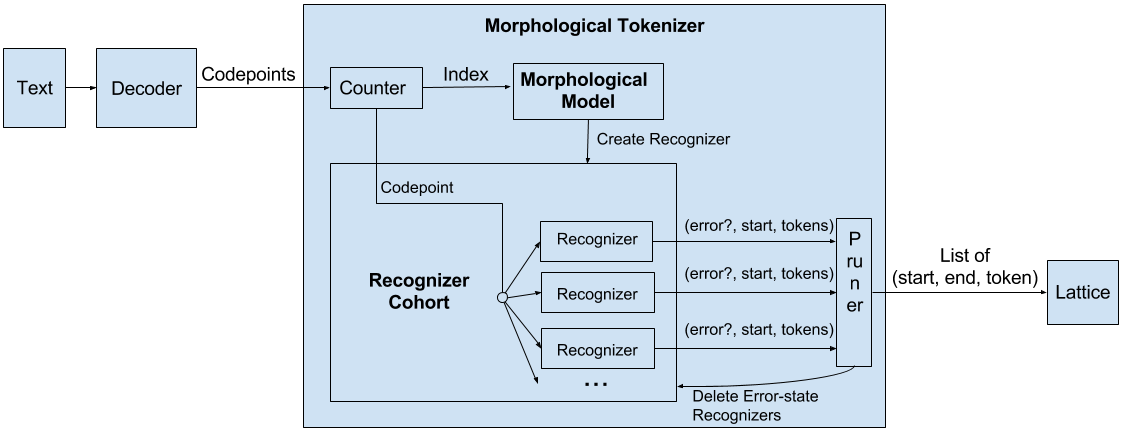
\includegraphics[width=\linewidth]{methodology/Morph}
	\caption{Morphological Tokenization}
	\label{morphdiagram}
\end{figure}

\subsection{Arabic}
I performed morphological tokenization of Arabic using the MADAMIRA morphological analyzer~\cite{pasha14}. MADAMIRA, unfortunately, does not expose an FSM network API, so it was necessary to collect complete candidate-token substrings to check all at once. Additionally, it does not provide any means of querying valid prefixes. In order to avoid quadratic or cubic runtime, which would make the experiment infeasible even on relatively short texts, extra rules were added to the interface connecting MADAMIRA to the generic tokenizer to reject strings satisfying certain conditions which I knew a priori could never result in valid prefixes. First, the interface would reject any string longer than 16 codepoints, as there were no tokens in the Arabic corpus greater than that length. Second, the interface would reject any string containing a whitespace codepoint, since I knew ahead of time that the MADAMIRA lexicon did not contain any tokens containing whitespace codepoints.
In other respects, however, MADAMIRA is almost \textit{too} sophisticated to effectively integrate with a tokenizer. In particular, MADAMIRA does not assume that the input will necessarily be a single word, and can analyze sentences with words in context; as a result, it does its own word breaking (by some apparently undocumented method), and can return positive results for input containing more than one token. In order to account for this, I filtered MADAMIRA's output to accept only those strings which MADAMIRA identified as containing exactly one ``word". Additionally, MADAMIRA will ``helpfully" ignore extraneous punctuation, leading it to produce valid analyses for words with, e.g., parentheses attached, as well as for the actual words themselves. I could find no principled way to avoid these spurious analyses.

MADAMIRA is accessed via an HTTP interface, which introduces significant input/output overhead. In order to maximize CPU usage, I split the corpus into three parts processed by three simultaneous instances of the tokenizer, each accessing a single MADAMIRA server process.

\subsection{English}
I performed morphological tokenization of English with the Englex morphological description of English~\cite{antworthenglex} developed for PC-KIMMO~\cite{koskenniemi84}. This model was run on a modified version of PyKIMMO\footnote{A Python implementation of the KIMMO two-level morphology algorithm.} known as Stream-KIMMO~\cite{kearsley13}, which already has the appropriate FSM-like interface and required no adaptation. While the system runs in linear time, however, the original PyKIMMO implementation was highly inefficient, and introduced an enormous constant-factor slowdown, proportional to the size of the lexicon, due to simulating an FSM by dynamically calculating transitions and new states by iterating over the entire plain-text lexicon on every codepoint. Re-implementing the core of PyKIMMO to construct a real FSM was not a viable option, but I was able to introduce several efficiency improvements which sped up the algorithm by approximately a factor of five; still, the relative slowness of this analyzer limited the quantity of text that could be processed from the OANC within a reasonable timeframe. The English morphological experiment thus terminated after approximately four days, once sufficient data was obtained. The 100,165 tokens processed constitute approximately 0.7\% of the approximately 15-million-word OANC covering a random selection of genres.

\subsection{Korean}
I performed morphological tokenization of Korean using the KLEX morphological analyzer developed for the Xerox Finite-State Tools (XFST). KLEX was originally designed to operate with input in either KSC-5601 or Unicode 1.0 encoding. In order to comply with modern versions of XFST, which only accept UTF-8 or Latin-1 encodings, and to enable it to work with the corpus which had been converted into UTF-8, I modified the KLEX source code to handle modern Unicode input. Fortunately, KLEX had been designed to transliterate Hangul into a modified Yale romanization for internal processing and back again; thus, updating it for modern encodings was a simple matter of running a search-and-replace on the file containing Hangul-Yale equivalencies to replace the old Korean codepoints with modern Unicode 8.0 UTF-8 codepoints.
Python bindings for the XFST library do exist which are supposed to directly expose the underlying FSM, allowing linear-time traversal. However, these tools have not been maintained, and I was unable to successfully install the software. Instead, I made use of a simpler Python API which exposes only the ``apply up" and ``apply down" functions of the morphological analyzer. As with MADAMIRA, I thus introduced special-case rules which rejected any string longer than 22 codepoints (again based on the maximum-length token known to exist in the corpus), and to reject any string containing whitespace, again based on prior knowledge that the KLEX lexicon contained no tokens containing whitespace.
KLEX has the ability to recognize certain suffixes and clitics in isolation, if they are prefixed with the tag ``\^{}DEP+" to indicate their status as bound (dependent) morphemes. Thus, in order to account for at least some possible variation in tokenization conventions, I ran two experiments with the morphological tokenizer on Korean: one which ignored dependents, and one which checked every possible token alone and with ``\^{}DEP+" prefixed.

\section{Statistical Tokenization}
In order to create a predictive model for statistical tokenization, I computed mutual information (MI) scores for every pair of codepoints present in each corpus. For this purpose, MI is given by the formula $\log_2(\frac{P(a,b)}{P(a)P(b)})$, where $a$ and $b$ are adjacent codepoints, $P(x)$ is the probability of encountering a given codepoint $x$ at any position, and $P(a,b)$ is the joint probability of encountering the pair of codepoints $a$ followed by $b$ at any given position. Word boundaries were then predicted by testing the MI score of each codepoint pair in the corpora against a threshold value, as shown in \ref{statdiagram}. This trivially requires constant time per pair, and thus achieves the necessary $O(n)$ complexity for on-line usage, like the morphological algorithm.

Two different methods of calculating thresholds were used in different experiments:
\begin{enumerate}
	\item In the gap-threshold method, the largest gap between MI scores for a given languages was identified, and a model was created which predicts a token boundary between every pair of codepoints whose mutual information score falls below that gap. This encodes the intuition that there may be a significant clustering of codepoint pairs that can occur across token boundaries versus codepoint pairs that tend to occur within tokens, and was previously found to produce extremely high recall with reasonable accuracy on English data~\cite{kearsley14}.
	\item In the zero-threshold method, boundaries are predicted between every pair of codepoints whose MI score is less than or equal to 0, for all languages. This encodes the intuition that there may be a token boundary wherever the probability of encountering a codepoint in that position is less than the overall probability of encountering that codepoint in any position.
\end{enumerate}
Contrary to Rytting's method~\cite{rytting04}, MI scores are used to predict token boundaries directly, rather than being weighted against a known prior probability of a particular codepoint pair marking a token boundary as determined from training data. This simplification results in a completely unsupervised system, which makes it attractive for use in a hybrid system as it avoids increasing the amount of language-specific configuration needed beyond the dictionary or morphological With either threshold-assignment method the model could also be updated on-line, as in Brent's prior work~\cite{brent99}, during real-time processing of a large input stream.

As in the morphological experiments, the output of each statistical experiment was saved to allow replaying the output for hybrid experiments. Since the statistical methods only identify single boundaries between tokens, rather than pairs bounding the start and end of a token, the saved output in this case consists of only a single list of possible boundary indices.

\begin{figure}
	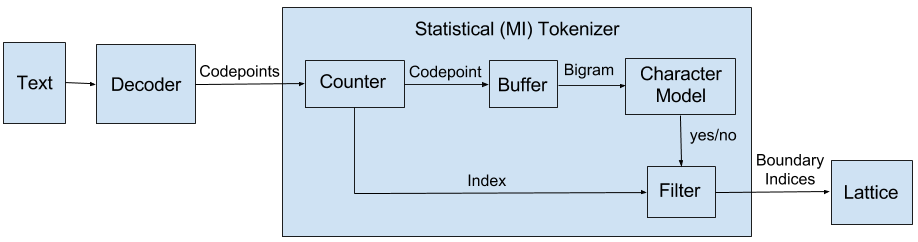
\includegraphics[width=\linewidth]{methodology/MI}
	\caption{Statistical Tokenization}
	\label{statdiagram}
\end{figure}

\section{Hybrid Tokenization}
I tested two methods of combining statistical and morphological methods to produce an improved hybrid tokenization system: ``filtering" and ``filling". Each of these was run with the output of both zero-threshold and gap-threshold statistical experiments, for a total of four hybrid experiments.

The filtering method is an attempt to improve system performance on precision by only initiating a new recognizer to add to the active cohort in the morphological tokenizer at indices where the statistical model indicates a token boundary is likely. This should eliminate spurious tokens that appear as suffixes of other tokens. This approach was simulated by constructing a new stream of (start, end) index pairs from stored morphological output including only those pairs in which the start index exists in the stored statistical data.

The filling method is an attempt to improve performance on recall and address the limitations of lexical-access based tokenization methods (including morphological tokenizers). This approach uses statistical predictions to fill in gaps of unanalyzed codepoints between tokens identified by the morphological model. This was simulated by identifying spans of codepoints not covered by any (start, end) pair in the morphological output, and filling them in with all (start, end) pairs that could be constructed from the predictions of the statistical models over those spans. One downside of this method is that, while it should run in amortized linear ($O(n)$) time in most cases, it does have worst-case quadratic ($O(n^2)$) performance on pathological inputs where the morphological model recognizes no possible tokens. As previously discussed, this would make it unsuitable for on-line usage. As long as the morphological model has reasonably good coverage, however, this should not become an issue in practice.

\begin{figure}
	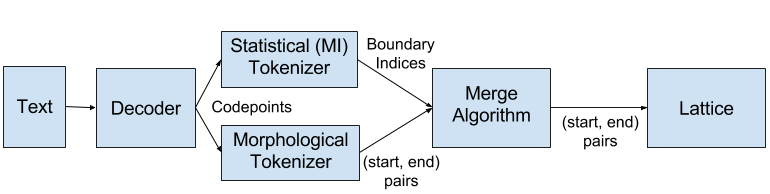
\includegraphics[width=\linewidth]{methodology/Hybrid}
	\caption{Hybrid Tokenization}
	\label{hybriddiagram}
\end{figure}

\section{Evaluation}
I evaluated all seven experiments on recognition of starting boundaries, ending boundaries, total boundaries (with no distinction between starting and ending), and matched pairs, representing specific tokens.

Since statistical predictions do not distinguish starting boundaries from ending boundaries, the precision measures for starting and ending boundaries considered individually are skewed, as they were determined by the total number of correctly-predicted boundaries that are starting (or ending) boundaries over the total number of undifferentiated boundaries predicted. This makes comparisons with the precision and F-scores for other methods slightly suspect. Recall, however, could be calculated normally for start and ending boundary predictions, and all three measures were calculated normally for the total set of individual boundaries. Token recall was based on the number of (start, end) pairs in the answer key for which both starting and ending indices appeared in the statistical output. Because the statistical tokenizers output only individual boundaries at a time, rather than (start, end) pairs bounding a single token, I omitted precision calculations for complete tokens for these experiments. The lack of pairing information makes precision measures on an un-pruned lattice (containing token hypotheses derived from all possible pairs of undistinguished boundaries) almost useless\textemdash the number of possible hypotheses for all possible pairs grows as the square of the input length, making precision measurements dependent almost entirely on the size of the input, rather than any inherent feature of the algorithm. In the absence of a precision value, F-score is also meaningless. In place of precision for complete tokens, I also evaluated statistical results on what fraction of all codepoint boundaries were identified as possible token boundaries; a lower score on this measure corresponds to a higher effective precision, in terms of reducing the amount of work required by later stages of an NLP pipeline.

For the morphological experiments, I calculated precision, recall, and F-score for all four types of output. Starting and ending boundary sets were merged into a single undifferentiated set to allow direct comparison on that measure with the purely statistical methods. With no generic method of controlling for the effects of differing effective token definitions between corpora and morphological analyzers, I obtained qualitative results by manual inspection of the lists of missed types and tokens for each language.

Since morphological tokenization depends on a morphological analyzer to identify lexical items and other valid tokens, my evaluation results for any particular language depend on the qualities of the analyzer available for that language. In particular, we can expect maximum accuracy and recall measurements when the definition of a ``token" used by the creator of a morphological analyzer is the same as the definition of a token used by the corpus annotator. Additionally, we can expect recall to be approximately bounded by the percentage of actual tokens in the corpus that are recognizable by the analyzer in isolation, with any missed tokens being restricted to those that are out-of-vocabulary for the analyzer.
In order to control for the quality of the analyzers used, I ran coverage tests to measure the fraction of tokens and types in the answer key that were recognizable by the analyzer for each language.

As in the morphological experiments, I calculated precision, recall, and F-score for starting boundaries, ending boundaries, total individual boundaries, and matched pairs for all hybrid experiments. I also calculated a reduction factor for the filter experiments, consisting of the total number of token boundaries output by the filtering algorithm divided by the number of boundaries present in the raw morphological output.